A IDE a ser usada para programar um STM32 é o TrueSTUDIO, distribuido pela Atollic, que forá adquirida pela STMicroelectronics em 2017
É um software livre para programar C/C++, criado com base na plataforma Eclipse, possui todas as funções esperadas para o trabalho com o STM32, como edição, compilação e debug.
Uma das vantagens do TrueSTUDIO é que não há limite para tamanho de projeto, o que o torna idela para trabalhos profissionais. O TrueSTUDIO parou de receber atualização em 2017, depois arquisição pela STMicroelectronics
\cite{apostila_microprossados}


\begin{figure}[h]
	\centering
	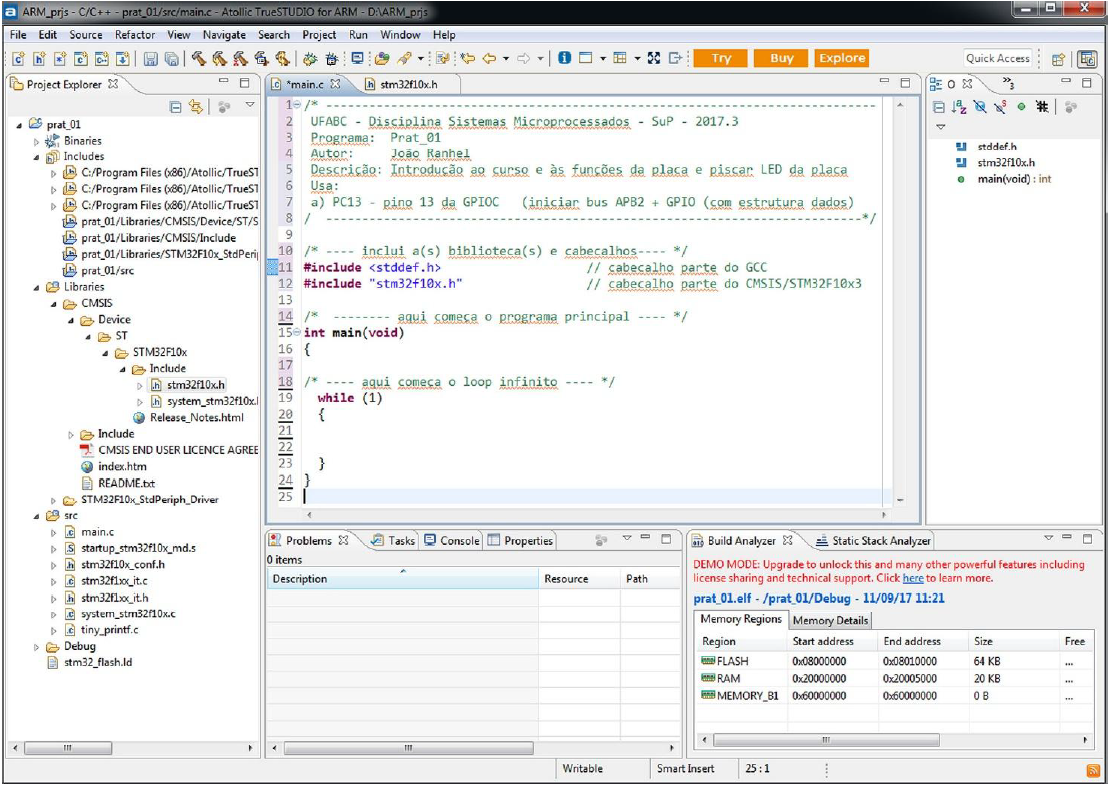
\includegraphics[width=0.8\textwidth]{figures/atollic}
	\caption{Interface Atollic \cite{apostila_microprossados}}
\end{figure}

